\documentclass{article}
\usepackage{assets/arxiv/arxiv}
% Disable 'A Preprint' label
\renewcommand{\headeright}{}
\renewcommand{\undertitle}{}
\usepackage{minted}
\usepackage{longtable}
\usepackage{listings}
\lstset{breaklines=true, columns=fullflexible}
\usepackage{fontspec}
% Use Source Sans Pro sans-serif font throughout
\usepackage[default]{sourcesanspro}
\usepackage{float}
\usepackage{amsmath}
\usepackage{caption}
\captionsetup{justification=raggedright,singlelinecheck=false}
\usepackage{lineno}
\usepackage{hyperref}
\linenumbers
\usepackage{pdflscape}
\usepackage{datetime2}
\usepackage{xr}
% spverbatim: verbatim with linewrap
\usepackage{spverbatim}

\title{Supplementary materials for \textit{Reporting Quality of Mendelian Randomization Studies Based on STROBE-MR: An Investigation Powered by Large Language Models}}
\usepackage{authblk}

\author[1,*]{[Jiangjie Zhou]}
\author[1,2,*]{[SECOND AUTHOR]}
\affil[1]{
  [DEPARTMENT/UNIT], [INSTITUTION],
  [CITY],
  [COUNTRY]}
\affil[2]{
  [SECOND AFFILIATION], [INSTITUTION],
  [CITY],
  [COUNTRY]}
\affil[*]{Corresponding author: [EMAIL1], [EMAIL2]}

\bibliographystyle{unsrt}

\usepackage{graphicx}
\usepackage{booktabs}
\usepackage{siunitx}
\usepackage{placeins}

% Adjust float placement parameters for better positioning
\renewcommand{\topfraction}{0.9}
\renewcommand{\bottomfraction}{0.9}
\renewcommand{\textfraction}{0.1}
\renewcommand{\floatpagefraction}{0.8}
\setcounter{topnumber}{3}
\setcounter{bottomnumber}{3}
\setcounter{totalnumber}{6}

% hide the text
\providecommand\hide{}
\renewcommand{\hide}[1]{}

% mark things in TODO
% Usage: \todo{message} or \todo[TAG]{message}
% Default tag is TODO if not specified
% Examples:
%   \todo{Fix this section} -> TODO: Fix this section
%   \todo[FIXME]{Revise argument} -> FIXME: Revise argument
\usepackage[dvipsnames]{xcolor}
\providecommand\todo{}
\renewcommand{\todo}[2][TODO]{\colorbox{yellow}{\textcolor{red}{\textbf{#1:}} #2}}

% Simple TODO marker without message
% Usage: \TODO
\providecommand\TODO{}
\renewcommand{\TODO}{\colorbox{yellow}{\textcolor{red}{\textbf{TODO}}}}


\renewcommand{\thesection}{S\arabic{section}}

% Section-based numbering for figures and tables (e.g., Table S1-1, Figure S2-3)
\usepackage{chngcntr}
\counterwithin{figure}{section}
\counterwithin{table}{section}
\renewcommand{\thefigure}{\thesection-\arabic{figure}}
\renewcommand{\thetable}{\thesection-\arabic{table}}

% NOTE: this is path to the aux file
\externaldocument{main-manuscript}

\begin{document}

\maketitle

\pagebreak

% ==== Optional: Glossary ====
% Uncomment to add a glossary defining key terms used in the manuscript.
% \section{Glossary} \label{sec:glossary}
% % Optional glossary section — define key terms used in the manuscript.
% Cross-reference sections where terms first appear or are discussed in depth.
% Remove this file and its \input in supplementary-materials.tex if not needed.

Here we describe the various terms used in the manuscript and reference the main sections
where these terms either first appear or are the topics for discussion.

\begin{itemize}

  \item \textbf{[TERM 1]}
    (Section~\ref{sec:[SECTION-LABEL]})
    [Definition of term 1.]

  \item \textbf{[TERM 2]}
    (Section~\ref{sec:[SECTION-LABEL]})
    [Definition of term 2.]

\end{itemize}

% \pagebreak

% \section{Additional methodology details} \label{sec:supp-methods}
% % Supplementary methodology details

\subsection{Detailed methodology} \label{subsec:supp-detailed-methods}

[Extended methodology descriptions that were too detailed for the main manuscript]

Here we cross-ref the main Section~\ref{sec:methods}

\subsection{Additional procedures}

[Additional procedural details]

% Example cross-reference back to main manuscript
% This methodology extends the approach described in Section~\ref{sec:methods} of the main manuscript.

% \pagebreak

% \section{Additional results and analysis} \label{sec:supp-results}
% % Supplementary results and analysis

\subsection{Additional analysis} \label{subsec:supp-additional-analysis}

[Additional results and analysis that support the main findings]

\subsection{Sensitivity analysis}

[Sensitivity analysis results]

% Example cross-reference back to main manuscript
% These results support the findings presented in Section~\ref{sec:results} of the main manuscript.
% \pagebreak

\section{Supplementary tables} \label{sec:supp-tables}
% Supplementary tables

\begin{longtable}{lllp{10cm}}
\caption{Definitions of STROBE-MR components}
\label{tab:def:component} \\

\toprule
Index & Section & Item & Component \\
\midrule
\endfirsthead

\toprule
Index & Section & Item & Component \\
\midrule
\endhead

\bottomrule
\endfoot

1 & Title and Abstract & 1 & Indicate Mendelian randomization (MR) as the study's design in the title and/or the abstract if that is a main purpose of the study \\
2 & Introduction & 2 & Explain the scientific background and rationale for the reported study. What is the exposure? Is a potential causal relationship between exposure and outcome plausible? Justify why MR is a helpful method to address the study question \\
3 & Introduction & 3 & State specific objectives clearly, including pre-specified causal hypotheses (if any). State that MR is a method that, under specific assumptions, intends to estimate causal effects \\
4 & Methods & 4 & Present data sources of the study early in the article \\
5 & Methods & 4 & Present 2. Methods of the study in the article \\
6 & Methods & 4 & Present 3. Exposures of the study in the article \\
7 & Methods & 4 & Present 4. Outcomes of the study in the article \\
8 & Methods & 4 & including a table listing sources of data for all phases of the study \\
9 & Methods & 4a & [Setting] For each data source, describe its study design \\
10 & Methods & 4a & [Setting] For each data source, describe its underlying population \\
11 & Methods & 4a & [Setting] For each data source,  describe its locations \\
12 & Methods & 4a & [Setting] For each data source, describe relevant dates, including periods of recruitment \\
13 & Methods & 4a & [Setting] For each data source, describe its exposure \\
14 & Methods & 4a & [Setting] For each data source, describe how the follow-up process was conducted  \\
15 & Methods & 4a & [Setting] For each data source, describe the data collection process \\
16 & Methods & 4b & [Paricipants] For each data source, give the eligibility criteria, and the sources and methods of selection of participants \\
17 & Methods & 4b & [Paricipants] For each data source, report the sample size \\
18 & Methods & 4b & [Paricipants] For each data source, report whether any power or sample size calculations were carried out prior to the main analysis \\
19 & Methods & 4c & [Paricipants] For each data source, describe measurement of genetic variants \\
20 & Methods & 4c & [Paricipants] For each data source,  describe quality control of genetic variants \\
21 & Methods & 4c & [Paricipants] For each data source, describe  selection of genetic variants \\
22 & Methods & 4d & Describe methods of assessment and diagnostic criteria for each exposure \\
23 & Methods & 4d & Describe methods of assessment and diagnostic criteria for each outcome \\
24 & Methods & 4d & Describe methods of assessment and diagnostic criteria for other relevant variables \\
25 & Methods & 4e & Provide details of ethics committee approval and participant informed consent, if relevant \\
26 & Methods & 5 & Explicitly state the relevance assumption of IV \\
27 & Methods & 5 & Explicitly state the independence assumption of IV \\
28 & Methods & 5 & Explicitly state the exclusion assumption of IV \\
29 & Methods & 5 & State assumptions for any additional or sensitivity analysis \\
30 & Methods & 6a & Describe how quantitative variables were handled in the analyses (i.e., scale, units, model) \\
31 & Methods & 6b & Describe how genetic variants were handled in the analyses and, if applicable, how their weights were selected \\
32 & Methods & 6c & Describe the MR estimator (e.g. two-stage least squares, Wald ratio) and related statistics. \\
33 & Methods & 6c & Detail the included covariates \\
34 & Methods & 6c & in case of two-sample MR, whether the same covariate set was used for adjustment in the two samples \\
35 & Methods & 6d & Explain how missing data were addressed \\
36 & Methods & 6e & If applicable, indicate how multiple testing was addressed \\
37 & Methods & 7 & Describe any methods or prior knowledge used to assess the relevance assumption of IV \\
38 & Methods & 7 & Describe any methods or prior knowledge used to assess the independence  assumption of IV \\
39 & Methods & 7 & Describe any methods or prior knowledge used to assess the exclusion assumption of IV \\
40 & Methods & 7 & Describe any methods or prior knowledge used to assess the assumptions for any additional analysis or sensitivity analysis \\
41 & Methods & 8 & Describe any sensitivity analyses or additional analyses performed \\
42 & Methods & 9a & Name statistical software and package(s), including version and settings used \\
43 & Methods & 9b & State whether the study protocol and details were pre-registered (as well as when and where) \\
44 & Results & 10a & Report the numbers of individuals at each stage of included studies and reasons for exclusion. Consider use of a flow diagram \\
45 & Results & 10b & Report summary statistics for phenotypic exposure(s), outcome(s), and other relevant variables (e.g. means, SDs, proportions) \\
46 & Results & 10c & If the data sources include meta-analyses of previous studies, provide the assessments of heterogeneity across these studies \\
47 & Results & 10d & For two-sample MR: Provide justification of the similarity of the genetic variant-exposure associations between the exposure and outcome samples \\
48 & Results & 10d & For two-sample MR: Provide information on the number of individuals who overlap between the exposure and outcome studies \\
49 & Results & 11a & Report the associations between genetic variant and exposure, and between genetic variant and outcome, preferably on an interpretable scale \\
50 & Results & 11b & Report MR estimates of the relationship between exposure and outcome, and the measures of uncertainty from the MR analysis, on an interpretable scale, such as odds ratio or relative risk per SD difference \\
51 & Results & 11c & Describe whether translating estimates of relative risk into absolute risk is conducted \\
52 & Results & 11d & Consider plots to visualize results (e.g. forest plot, scatterplot of associations between genetic variants and outcome versus between genetic variants and exposure) \\
53 & Results & 12a & Report results of the assessment of the relevance assumption \\
54 & Results & 12a & Report results of the assessment of the independence assumption \\
55 & Results & 12a & Report results of the assessment of the exclusion assumption \\
56 & Results & 12a & Report results of the assessment of the any additional assumption, if relevant  \\
57 & Results & 12b & Report any additional statistics \\
58 & Results & 13a & Report results from any sensitivity analyses to assess the robustness of the main results to violations of the assumptions \\
59 & Results & 13b & Report results from other sensitivity analyses or additional analyses \\
60 & Results & 13c & Report any assessment of direction of causal relationship (e.g., bidirectional MR) \\
61 & Results & 13d & Report and compare with estimates from non-MR analyses \\
62 & Results & 13e & Consider additional plots to visualize results (e.g., leave-one-out analyses) \\
63 & Discussion & 14 & Summarize key results with reference to study objectives \\
64 & Discussion & 15 & Limitation: discuss the validity of the IV assumptions \\
65 & Discussion & 15 & Limitation: discuss other sources of potential bias and imprecision \\
66 & Discussion & 15 & Limitation: discuss both direction and magnitude of any potential bias and any efforts to address them \\
67 & Discussion & 16a & Meaning: Give a cautious overall interpretation of results in the context of their limitations and in comparison with other studies \\
68 & Discussion & 16b & Mechanism: Discuss underlying biological mechanisms that could drive a potential causal relationship between the investigated exposure and the outcome \\
69 & Discussion & 16b & Mechanism: Discuss whether the gene-environment equivalence assumption is reasonable \\
70 & Discussion & 16b & Mechanism: Clarifying that IV estimates may provide causal effects only under certain assumptions  \\
71 & Discussion & 16c & Clinical relevance: Discuss whether the results have clinical or public policy relevance, and to what extent they inform effect sizes of possible interventions \\
72 & Discussion & 17 & Discuss the generalizability of the study results to other populations \\
73 & Discussion & 17 & Discuss the generalizability of the study results across other exposure periods/timings \\
74 & Discussion & 17 & Discuss the generalizability of the study results across other levels of exposure \\
75 & Other Information & 18 & Describe sources of funding in the present study \\
76 & Other Information & 18 & Describe  the role of funders in the present study \\
77 & Other Information & 18 & If applicable, describe sources of funding for the databases or studies on which the present study is based \\
78 & Other Information & 19 & Provide the data used to perform all analyses or report where and how the data can be accessed, and reference these sources in the article \\
79 & Other Information & 19 & Provide the statistical code needed to reproduce the results in the article, or report whether the code is publicly accessible and if so, where \\
80 & Other Information & 20 & All authors should declare all potential conflicts of interest \\

\end{longtable}


\begin{table}[h]
    \caption{API parameters for OpenAI platform}
    \begin{tabular}{lp{8cm}}
    \hline
    Parameter & Value \\
    \hline
    text\_format &
\begin{verbatim}
class Assessment(BaseModel): 
    index: int 
    rationale: str 
    relevant_text: str = "" 
    status: int
\end{verbatim} 
\\
    reasoning\_effort & "high" \\
    \hline
    \end{tabular}
    \label{tab:params:openai}
\end{table}

\begin{table}[h]
    \centering
    \caption{Definition of JSON object}
    \label{tab:json}
    \begin{tabular}{l l}
    \hline
    Field   &   Explanation \\
    \hline
    pmcid  &  PMCID \\
    title   &   title of the article \\
    year    &   publication year \\
    abstract    &   abstract of the article \\
    keyword &   keywords of the article \\
    sections    &   sections in the main text \\
    figures & links of figures included in the main text\\
    attachments & links of attachment files\\
    \hline
    \end{tabular}
\end{table}

\begin{longtable}{rllllllll}
\caption{Annotation summary by component}
\label{tab:eval:component} \\

\toprule
Index & Section & Item & Reported(JZ) & Not Reported(JZ) & Reported(YW) & Not Reported(YW) & Disagreement \\
\midrule
\endfirsthead

\toprule
Index & Section & Item & Reported(JZ) & Not Reported(JZ) & Reported(YW) & Not Reported(YW) & Disagreement \\
\midrule
\endhead

\bottomrule
\endfoot

1 & Title and Abstract & 1 & 46 & 0 & 46 & 0 & 0 \\
2 & Introduction & 2 & 46 & 0 & 46 & 0 & 0 \\
3 & Introduction & 3 & 42 & 4 & 43 & 3 & 1 \\
4 & Methods & 4 & 46 & 0 & 46 & 0 & 0 \\
5 & Methods & 4 & 46 & 0 & 46 & 0 & 0 \\
6 & Methods & 4 & 46 & 0 & 46 & 0 & 0 \\
7 & Methods & 4 & 46 & 0 & 46 & 0 & 0 \\
8 & Methods & 4 & 27 & 19 & 27 & 19 & 2 \\
9 & Methods & 4a & 24 & 22 & 28 & 18 & 6 \\
10 & Methods & 4a & 36 & 10 & 39 & 7 & 7 \\
11 & Methods & 4a & 26 & 20 & 23 & 23 & 9 \\
12 & Methods & 4a & 11 & 35 & 7 & 39 & 4 \\
13 & Methods & 4a & 38 & 8 & 36 & 10 & 4 \\
14 & Methods & 4a & 5 & 32 & 6 & 21 & 18 \\
15 & Methods & 4a & 16 & 30 & 19 & 27 & 9 \\
16 & Methods & 4b & 10 & 36 & 10 & 36 & 2 \\
17 & Methods & 4b & 43 & 3 & 44 & 2 & 1 \\
18 & Methods & 4b & 4 & 42 & 7 & 39 & 3 \\
19 & Methods & 4c & 16 & 30 & 13 & 32 & 12 \\
20 & Methods & 4c & 16 & 30 & 11 & 35 & 15 \\
21 & Methods & 4c & 46 & 0 & 46 & 0 & 0 \\
22 & Methods & 4d & 29 & 17 & 28 & 18 & 1 \\
23 & Methods & 4d & 24 & 22 & 26 & 20 & 4 \\
24 & Methods & 4d & 13 & 33 & 16 & 30 & 5 \\
25 & Methods & 4e & 40 & 5 & 41 & 4 & 6 \\
26 & Methods & 5 & 32 & 14 & 37 & 9 & 5 \\
27 & Methods & 5 & 32 & 14 & 35 & 11 & 3 \\
28 & Methods & 5 & 32 & 14 & 35 & 11 & 3 \\
29 & Methods & 5 & 8 & 38 & 8 & 38 & 2 \\
30 & Methods & 6a & 19 & 23 & 16 & 30 & 7 \\
31 & Methods & 6b & 44 & 2 & 42 & 4 & 2 \\
32 & Methods & 6c & 46 & 0 & 46 & 0 & 0 \\
33 & Methods & 6c & 15 & 31 & 15 & 31 & 2 \\
34 & Methods & 6c & 3 & 40 & 2 & 41 & 1 \\
35 & Methods & 6d & 5 & 41 & 6 & 40 & 5 \\
36 & Methods & 6e & 24 & 22 & 23 & 23 & 1 \\
37 & Methods & 7 & 42 & 4 & 41 & 5 & 1 \\
38 & Methods & 7 & 24 & 22 & 30 & 16 & 6 \\
39 & Methods & 7 & 43 & 3 & 44 & 2 & 3 \\
40 & Methods & 7 & 18 & 28 & 38 & 8 & 20 \\
41 & Methods & 8 & 46 & 0 & 46 & 0 & 0 \\
42 & Methods & 9a & 23 & 23 & 19 & 27 & 14 \\
43 & Methods & 9b & 3 & 43 & 3 & 43 & 0 \\
44 & Results & 10a & 14 & 31 & 16 & 29 & 2 \\
45 & Results & 10b & 16 & 30 & 18 & 28 & 6 \\
46 & Results & 10c & 4 & 17 & 5 & 31 & 16 \\
47 & Results & 10d & 19 & 24 & 12 & 31 & 7 \\
48 & Results & 10d & 6 & 37 & 6 & 37 & 0 \\
49 & Results & 11a & 33 & 13 & 33 & 13 & 2 \\
50 & Results & 11b & 45 & 1 & 46 & 0 & 1 \\
51 & Results & 11c & 0 & 46 & 0 & 45 & 1 \\
52 & Results & 11d & 45 & 1 & 46 & 0 & 1 \\
53 & Results & 12a & 37 & 9 & 36 & 10 & 3 \\
54 & Results & 12a & 24 & 22 & 32 & 14 & 8 \\
55 & Results & 12a & 43 & 3 & 46 & 0 & 3 \\
56 & Results & 12a & 16 & 30 & 26 & 20 & 10 \\
57 & Results & 12b & 42 & 4 & 42 & 4 & 0 \\
58 & Results & 13a & 45 & 1 & 46 & 0 & 1 \\
59 & Results & 13b & 44 & 2 & 43 & 3 & 3 \\
60 & Results & 13c & 17 & 28 & 17 & 27 & 1 \\
61 & Results & 13d & 19 & 27 & 15 & 30 & 17 \\
62 & Results & 13e & 35 & 11 & 30 & 16 & 7 \\
63 & Discussion & 14 & 46 & 0 & 46 & 0 & 0 \\
64 & Discussion & 15 & 37 & 9 & 40 & 6 & 3 \\
65 & Discussion & 15 & 45 & 1 & 44 & 2 & 1 \\
66 & Discussion & 15 & 30 & 16 & 36 & 10 & 6 \\
67 & Discussion & 16a & 46 & 0 & 46 & 0 & 0 \\
68 & Discussion & 16b & 46 & 0 & 46 & 0 & 0 \\
69 & Discussion & 16b & 9 & 37 & 10 & 36 & 1 \\
70 & Discussion & 16b & 40 & 6 & 42 & 4 & 2 \\
71 & Discussion & 16c & 46 & 0 & 46 & 0 & 0 \\
72 & Discussion & 17 & 41 & 5 & 41 & 5 & 0 \\
73 & Discussion & 17 & 12 & 34 & 17 & 29 & 5 \\
74 & Discussion & 17 & 8 & 38 & 10 & 36 & 2 \\
75 & Other Information & 18 & 40 & 6 & 45 & 1 & 7 \\
76 & Other Information & 18 & 7 & 38 & 7 & 34 & 5 \\
77 & Other Information & 18 & 3 & 42 & 3 & 41 & 3 \\
78 & Other Information & 19 & 44 & 2 & 45 & 1 & 3 \\
79 & Other Information & 19 & 3 & 43 & 3 & 43 & 2 \\
80 & Other Information & 20 & 38 & 8 & 45 & 1 & 7 \\

\end{longtable}

\begin{longtable}{rllr}
\caption{Model accuracy by component}
\label{tab:model:accuracy} \\

\toprule
Index & Section & Item & Accuracy, \% \\
\midrule
\endfirsthead

\toprule
Index & Section & Item & Accuracy, \% \\
\midrule
\endhead

\bottomrule
\endfoot

1 & Title and Abstract & 1 & 100.0 \\
2 & Introduction & 2 & 100.0 \\
3 & Introduction & 3 & 91.3 \\
4 & Methods & 4 & 100.0 \\
5 & Methods & 4 & 100.0 \\
6 & Methods & 4 & 100.0 \\
7 & Methods & 4 & 97.8 \\
8 & Methods & 4 & 93.5 \\
9 & Methods & 4a & 76.1 \\
10 & Methods & 4a & 91.3 \\
11 & Methods & 4a & 80.4 \\
12 & Methods & 4a & 95.7 \\
13 & Methods & 4a & 78.3 \\
14 & Methods & 4a & 60.9 \\
15 & Methods & 4a & 84.8 \\
16 & Methods & 4b & 93.5 \\
17 & Methods & 4b & 91.3 \\
18 & Methods & 4b & 91.3 \\
19 & Methods & 4c & 69.6 \\
20 & Methods & 4c & 71.7 \\
21 & Methods & 4c & 100.0 \\
22 & Methods & 4d & 82.6 \\
23 & Methods & 4d & 91.3 \\
24 & Methods & 4d & 84.8 \\
25 & Methods & 4e & 80.4 \\
26 & Methods & 5 & 82.6 \\
27 & Methods & 5 & 87.0 \\
28 & Methods & 5 & 89.1 \\
29 & Methods & 5 & 89.1 \\
30 & Methods & 6a & 97.8 \\
31 & Methods & 6b & 71.7 \\
32 & Methods & 6c & 100.0 \\
33 & Methods & 6c & 97.8 \\
34 & Methods & 6c & 100.0 \\
35 & Methods & 6d & 91.3 \\
36 & Methods & 6e & 95.7 \\
37 & Methods & 7 & 91.3 \\
38 & Methods & 7 & 87.0 \\
39 & Methods & 7 & 97.8 \\
40 & Methods & 7 & 65.2 \\
41 & Methods & 8 & 100.0 \\
42 & Methods & 9a & 76.1 \\
43 & Methods & 9b & 97.8 \\
44 & Results & 10a & 76.1 \\
45 & Results & 10b & 82.6 \\
46 & Results & 10c & 71.7 \\
47 & Results & 10d & 60.9 \\
48 & Results & 10d & 97.8 \\
49 & Results & 11a & 78.3 \\
50 & Results & 11b & 97.8 \\
51 & Results & 11c & 95.7 \\
52 & Results & 11d & 91.3 \\
53 & Results & 12a & 93.5 \\
54 & Results & 12a & 82.6 \\
55 & Results & 12a & 95.7 \\
56 & Results & 12a & 63.0 \\
57 & Results & 12b & 89.1 \\
58 & Results & 13a & 100.0 \\
59 & Results & 13b & 100.0 \\
60 & Results & 13c & 73.9 \\
61 & Results & 13d & 65.2 \\
62 & Results & 13e & 76.1 \\
63 & Discussion & 14 & 100.0 \\
64 & Discussion & 15 & 93.5 \\
65 & Discussion & 15 & 100.0 \\
66 & Discussion & 15 & 82.6 \\
67 & Discussion & 16a & 100.0 \\
68 & Discussion & 16b & 100.0 \\
69 & Discussion & 16b & 91.3 \\
70 & Discussion & 16b & 91.3 \\
71 & Discussion & 16c & 100.0 \\
72 & Discussion & 17 & 97.8 \\
73 & Discussion & 17 & 89.1 \\
74 & Discussion & 17 & 84.8 \\
75 & Other Information & 18 & 93.5 \\
76 & Other Information & 18 & 100.0 \\
77 & Other Information & 18 & 97.8 \\
78 & Other Information & 19 & 93.5 \\
79 & Other Information & 19 & 97.8 \\
80 & Other Information & 20 & 89.1 \\

\end{longtable}

\begin{longtable}{lllllll}
\caption{STROBE-MR reporting by component}
\label{tab:report:component} \\

\toprule
Index & Section & Item & Reported, n(\%) & Not Reported, n(\%) & Not Applicablen, n(\%) \\
\midrule
\endfirsthead

\toprule
Index & Section & Item & Reported, n(\%) & Not Reported, n(\%) & Not Applicable, n(\%) \\
\midrule
\endhead

\bottomrule
\endfoot

1 & Title and Abstract & 1 & 12407 (97.7\%) & 187 (1.5\%) & 105 (0.8\%) \\
2 & Introduction & 2 & 12318 (97.0\%) & 336 (2.6\%) & 45 (0.4\%) \\
3 & Introduction & 3 & 11930 (93.9\%) & 716 (5.6\%) & 53 (0.4\%) \\
4 & Methods & 4 & 12543 (98.8\%) & 133 (1.0\%) & 23 (0.2\%) \\
5 & Methods & 4 & 12530 (98.7\%) & 146 (1.1\%) & 23 (0.2\%) \\
6 & Methods & 4 & 12532 (98.7\%) & 124 (1.0\%) & 43 (0.3\%) \\
7 & Methods & 4 & 12564 (98.9\%) & 89 (0.7\%) & 46 (0.4\%) \\
8 & Methods & 4 & 7016 (55.2\%) & 5644 (44.4\%) & 39 (0.3\%) \\
9 & Methods & 4a & 7917 (62.3\%) & 4749 (37.4\%) & 33 (0.3\%) \\
10 & Methods & 4a & 10474 (82.5\%) & 2189 (17.2\%) & 36 (0.3\%) \\
11 & Methods & 4a & 7823 (61.6\%) & 4824 (38.0\%) & 52 (0.4\%) \\
12 & Methods & 4a & 1860 (14.6\%) & 10790 (85.0\%) & 49 (0.4\%) \\
13 & Methods & 4a & 9393 (74.0\%) & 3264 (25.7\%) & 42 (0.3\%) \\
14 & Methods & 4a & 1555 (12.2\%) & 3326 (26.2\%) & 7818 (61.6\%) \\
15 & Methods & 4a & 7210 (56.8\%) & 5460 (43.0\%) & 29 (0.2\%) \\
16 & Methods & 4b & 4121 (32.5\%) & 8541 (67.3\%) & 37 (0.3\%) \\
17 & Methods & 4b & 11422 (89.9\%) & 1256 (9.9\%) & 21 (0.2\%) \\
18 & Methods & 4b & 1617 (12.7\%) & 11049 (87.0\%) & 33 (0.3\%) \\
19 & Methods & 4c & 5805 (45.7\%) & 6803 (53.6\%) & 91 (0.7\%) \\
20 & Methods & 4c & 8160 (64.3\%) & 4434 (34.9\%) & 105 (0.8\%) \\
21 & Methods & 4c & 11956 (94.1\%) & 653 (5.1\%) & 90 (0.7\%) \\
22 & Methods & 4d & 7461 (58.8\%) & 5187 (40.8\%) & 51 (0.4\%) \\
23 & Methods & 4d & 6699 (52.8\%) & 5951 (46.9\%) & 49 (0.4\%) \\
24 & Methods & 4d & 5505 (43.3\%) & 7106 (56.0\%) & 88 (0.7\%) \\
25 & Methods & 4e & 9537 (75.1\%) & 3064 (24.1\%) & 98 (0.8\%) \\
26 & Methods & 5 & 9918 (78.1\%) & 2660 (20.9\%) & 121 (1.0\%) \\
27 & Methods & 5 & 9279 (73.1\%) & 3299 (26.0\%) & 121 (1.0\%) \\
28 & Methods & 5 & 9394 (74.0\%) & 3184 (25.1\%) & 121 (1.0\%) \\
29 & Methods & 5 & 2008 (15.8\%) & 10548 (83.1\%) & 143 (1.1\%) \\
30 & Methods & 6a & 5620 (44.3\%) & 7045 (55.5\%) & 34 (0.3\%) \\
31 & Methods & 6b & 10289 (81.0\%) & 2311 (18.2\%) & 99 (0.8\%) \\
32 & Methods & 6c & 12163 (95.8\%) & 391 (3.1\%) & 145 (1.1\%) \\
33 & Methods & 6c & 4622 (36.4\%) & 8031 (63.2\%) & 46 (0.4\%) \\
34 & Methods & 6c & 454 (3.6\%) & 11309 (89.1\%) & 936 (7.4\%) \\
35 & Methods & 6d & 2023 (15.9\%) & 10620 (83.6\%) & 56 (0.4\%) \\
36 & Methods & 6e & 6048 (47.6\%) & 6545 (51.5\%) & 106 (0.8\%) \\
37 & Methods & 7 & 11040 (86.9\%) & 1540 (12.1\%) & 119 (0.9\%) \\
38 & Methods & 7 & 7950 (62.6\%) & 4630 (36.5\%) & 119 (0.9\%) \\
39 & Methods & 7 & 11736 (92.4\%) & 844 (6.6\%) & 119 (0.9\%) \\
40 & Methods & 7 & 10182 (80.2\%) & 2371 (18.7\%) & 146 (1.1\%) \\
41 & Methods & 8 & 12271 (96.6\%) & 391 (3.1\%) & 37 (0.3\%) \\
42 & Methods & 9a & 7509 (59.1\%) & 5172 (40.7\%) & 18 (0.1\%) \\
43 & Methods & 9b & 304 (2.4\%) & 12377 (97.5\%) & 18 (0.1\%) \\
44 & Results & 10a & 5997 (47.2\%) & 6666 (52.5\%) & 36 (0.3\%) \\
45 & Results & 10b & 4615 (36.3\%) & 8046 (63.4\%) & 38 (0.3\%) \\
46 & Results & 10c & 1215 (9.6\%) & 8104 (63.8\%) & 3380 (26.6\%) \\
47 & Results & 10d & 4169 (32.8\%) & 7637 (60.1\%) & 893 (7.0\%) \\
48 & Results & 10d & 2083 (16.4\%) & 9737 (76.7\%) & 879 (6.9\%) \\
49 & Results & 11a & 8403 (66.2\%) & 4186 (33.0\%) & 110 (0.9\%) \\
50 & Results & 11b & 11607 (91.4\%) & 938 (7.4\%) & 154 (1.2\%) \\
51 & Results & 11c & 269 (2.1\%) & 11738 (92.4\%) & 692 (5.4\%) \\
52 & Results & 11d & 11626 (91.6\%) & 1021 (8.0\%) & 52 (0.4\%) \\
53 & Results & 12a & 9093 (71.6\%) & 3480 (27.4\%) & 126 (1.0\%) \\
54 & Results & 12a & 7080 (55.8\%) & 5493 (43.3\%) & 126 (1.0\%) \\
55 & Results & 12a & 11250 (88.6\%) & 1323 (10.4\%) & 126 (1.0\%) \\
56 & Results & 12a & 6963 (54.8\%) & 5440 (42.8\%) & 296 (2.3\%) \\
57 & Results & 12b & 9670 (76.1\%) & 2785 (21.9\%) & 244 (1.9\%) \\
58 & Results & 13a & 12052 (94.9\%) & 585 (4.6\%) & 62 (0.5\%) \\
59 & Results & 13b & 11848 (93.3\%) & 795 (6.3\%) & 56 (0.4\%) \\
60 & Results & 13c & 5903 (46.5\%) & 4888 (38.5\%) & 1908 (15.0\%) \\
61 & Results & 13d & 8303 (65.4\%) & 4233 (33.3\%) & 163 (1.3\%) \\
62 & Results & 13e & 7919 (62.4\%) & 4473 (35.2\%) & 307 (2.4\%) \\
63 & Discussion & 14 & 12587 (99.1\%) & 88 (0.7\%) & 24 (0.2\%) \\
64 & Discussion & 15 & 9251 (72.8\%) & 3344 (26.3\%) & 104 (0.8\%) \\
65 & Discussion & 15 & 11969 (94.3\%) & 712 (5.6\%) & 18 (0.1\%) \\
66 & Discussion & 15 & 9686 (76.3\%) & 2995 (23.6\%) & 18 (0.1\%) \\
67 & Discussion & 16a & 12416 (97.8\%) & 263 (2.1\%) & 20 (0.2\%) \\
68 & Discussion & 16b & 12387 (97.5\%) & 259 (2.0\%) & 53 (0.4\%) \\
69 & Discussion & 16b & 1260 (9.9\%) & 11320 (89.1\%) & 119 (0.9\%) \\
70 & Discussion & 16b & 10754 (84.7\%) & 1839 (14.5\%) & 106 (0.8\%) \\
71 & Discussion & 16c & 12323 (97.0\%) & 344 (2.7\%) & 32 (0.3\%) \\
72 & Discussion & 17 & 10872 (85.6\%) & 1805 (14.2\%) & 22 (0.2\%) \\
73 & Discussion & 17 & 3314 (26.1\%) & 9329 (73.5\%) & 56 (0.4\%) \\
74 & Discussion & 17 & 2534 (20.0\%) & 10108 (79.6\%) & 57 (0.4\%) \\
75 & Other Information & 18 & 10586 (83.4\%) & 2101 (16.5\%) & 12 (0.1\%) \\
76 & Other Information & 18 & 3087 (24.3\%) & 9531 (75.1\%) & 81 (0.6\%) \\
77 & Other Information & 18 & 1802 (14.2\%) & 10791 (85.0\%) & 106 (0.8\%) \\
78 & Other Information & 19 & 11719 (92.3\%) & 965 (7.6\%) & 15 (0.1\%) \\
79 & Other Information & 19 & 1541 (12.1\%) & 11145 (87.8\%) & 13 (0.1\%) \\
80 & Other Information & 20 & 10689 (84.2\%) & 1998 (15.7\%) & 12 (0.1\%) \\

\end{longtable}
\pagebreak

\section{Supplementary figures} \label{sec:supp-figures}
% Supplementary figures

% \begin{figure}[H]
% \centering
% % Example figure placeholder
% \fbox{\parbox{0.7\textwidth}{
% \centering
% \vspace{2cm}
% [Figure placeholder]\\
% Include your figure here using:\\
% \texttt{\textbackslash includegraphics[width=\textbackslash textwidth]\{assets/figures/figure-name.pdf\}}
% \vspace{2cm}
% }}
% \caption{Example supplementary figure caption}
% \label{fig:supp-example}
% \end{figure}


\begin{figure}[H]
    \centering
    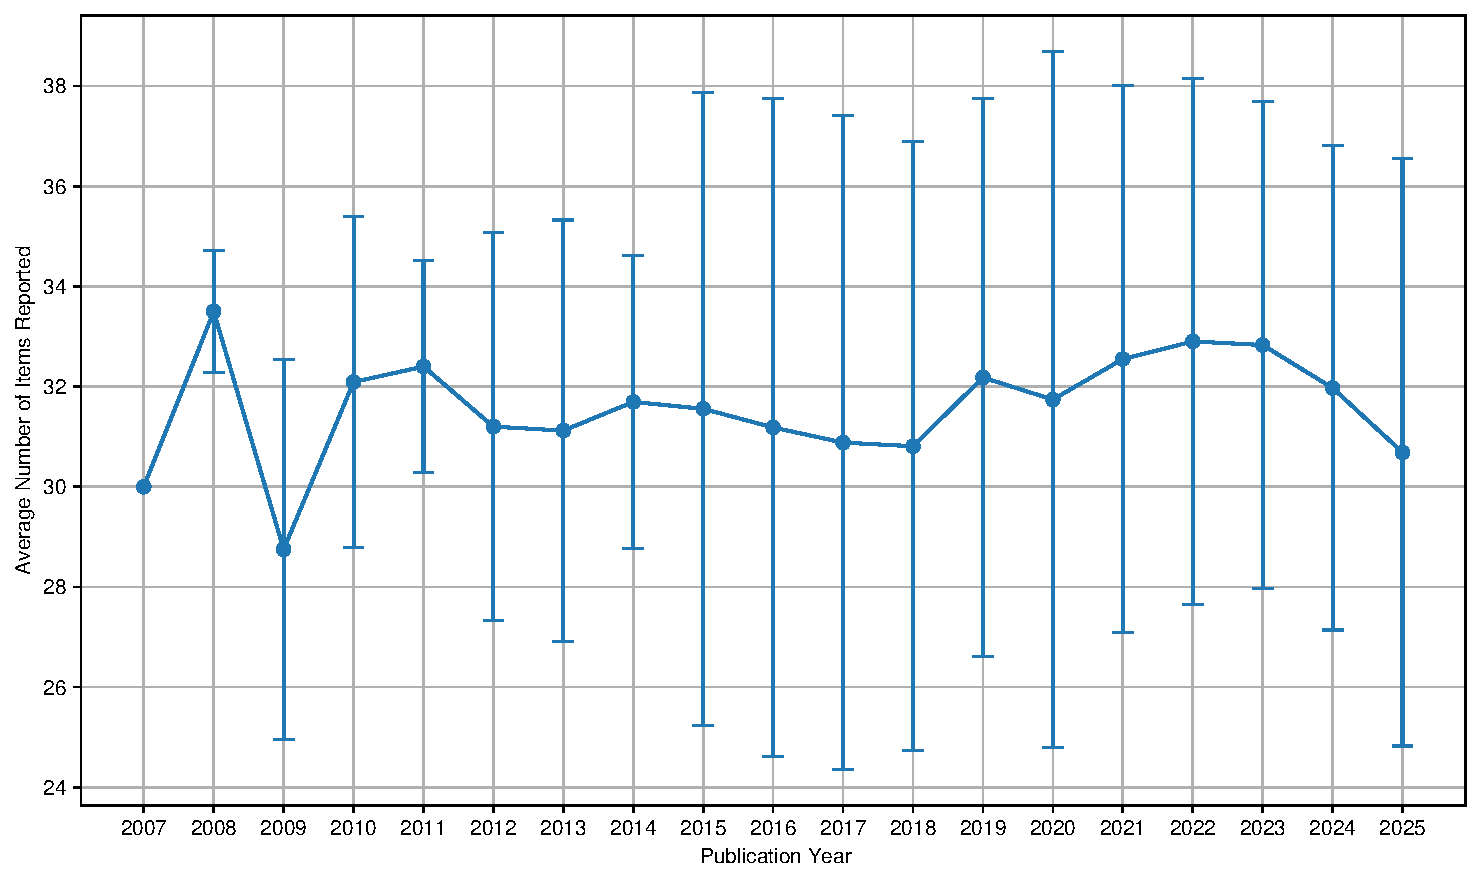
\includegraphics[width=0.8\linewidth]{assets/figures/subitem_any/avg_meet_num_by_year.pdf}
    \caption{Sensitivity analysis: STROBE-MR reporting by publication year}
    \label{append:fig:meet:year}
\end{figure}

\begin{figure}[H]
    \centering
    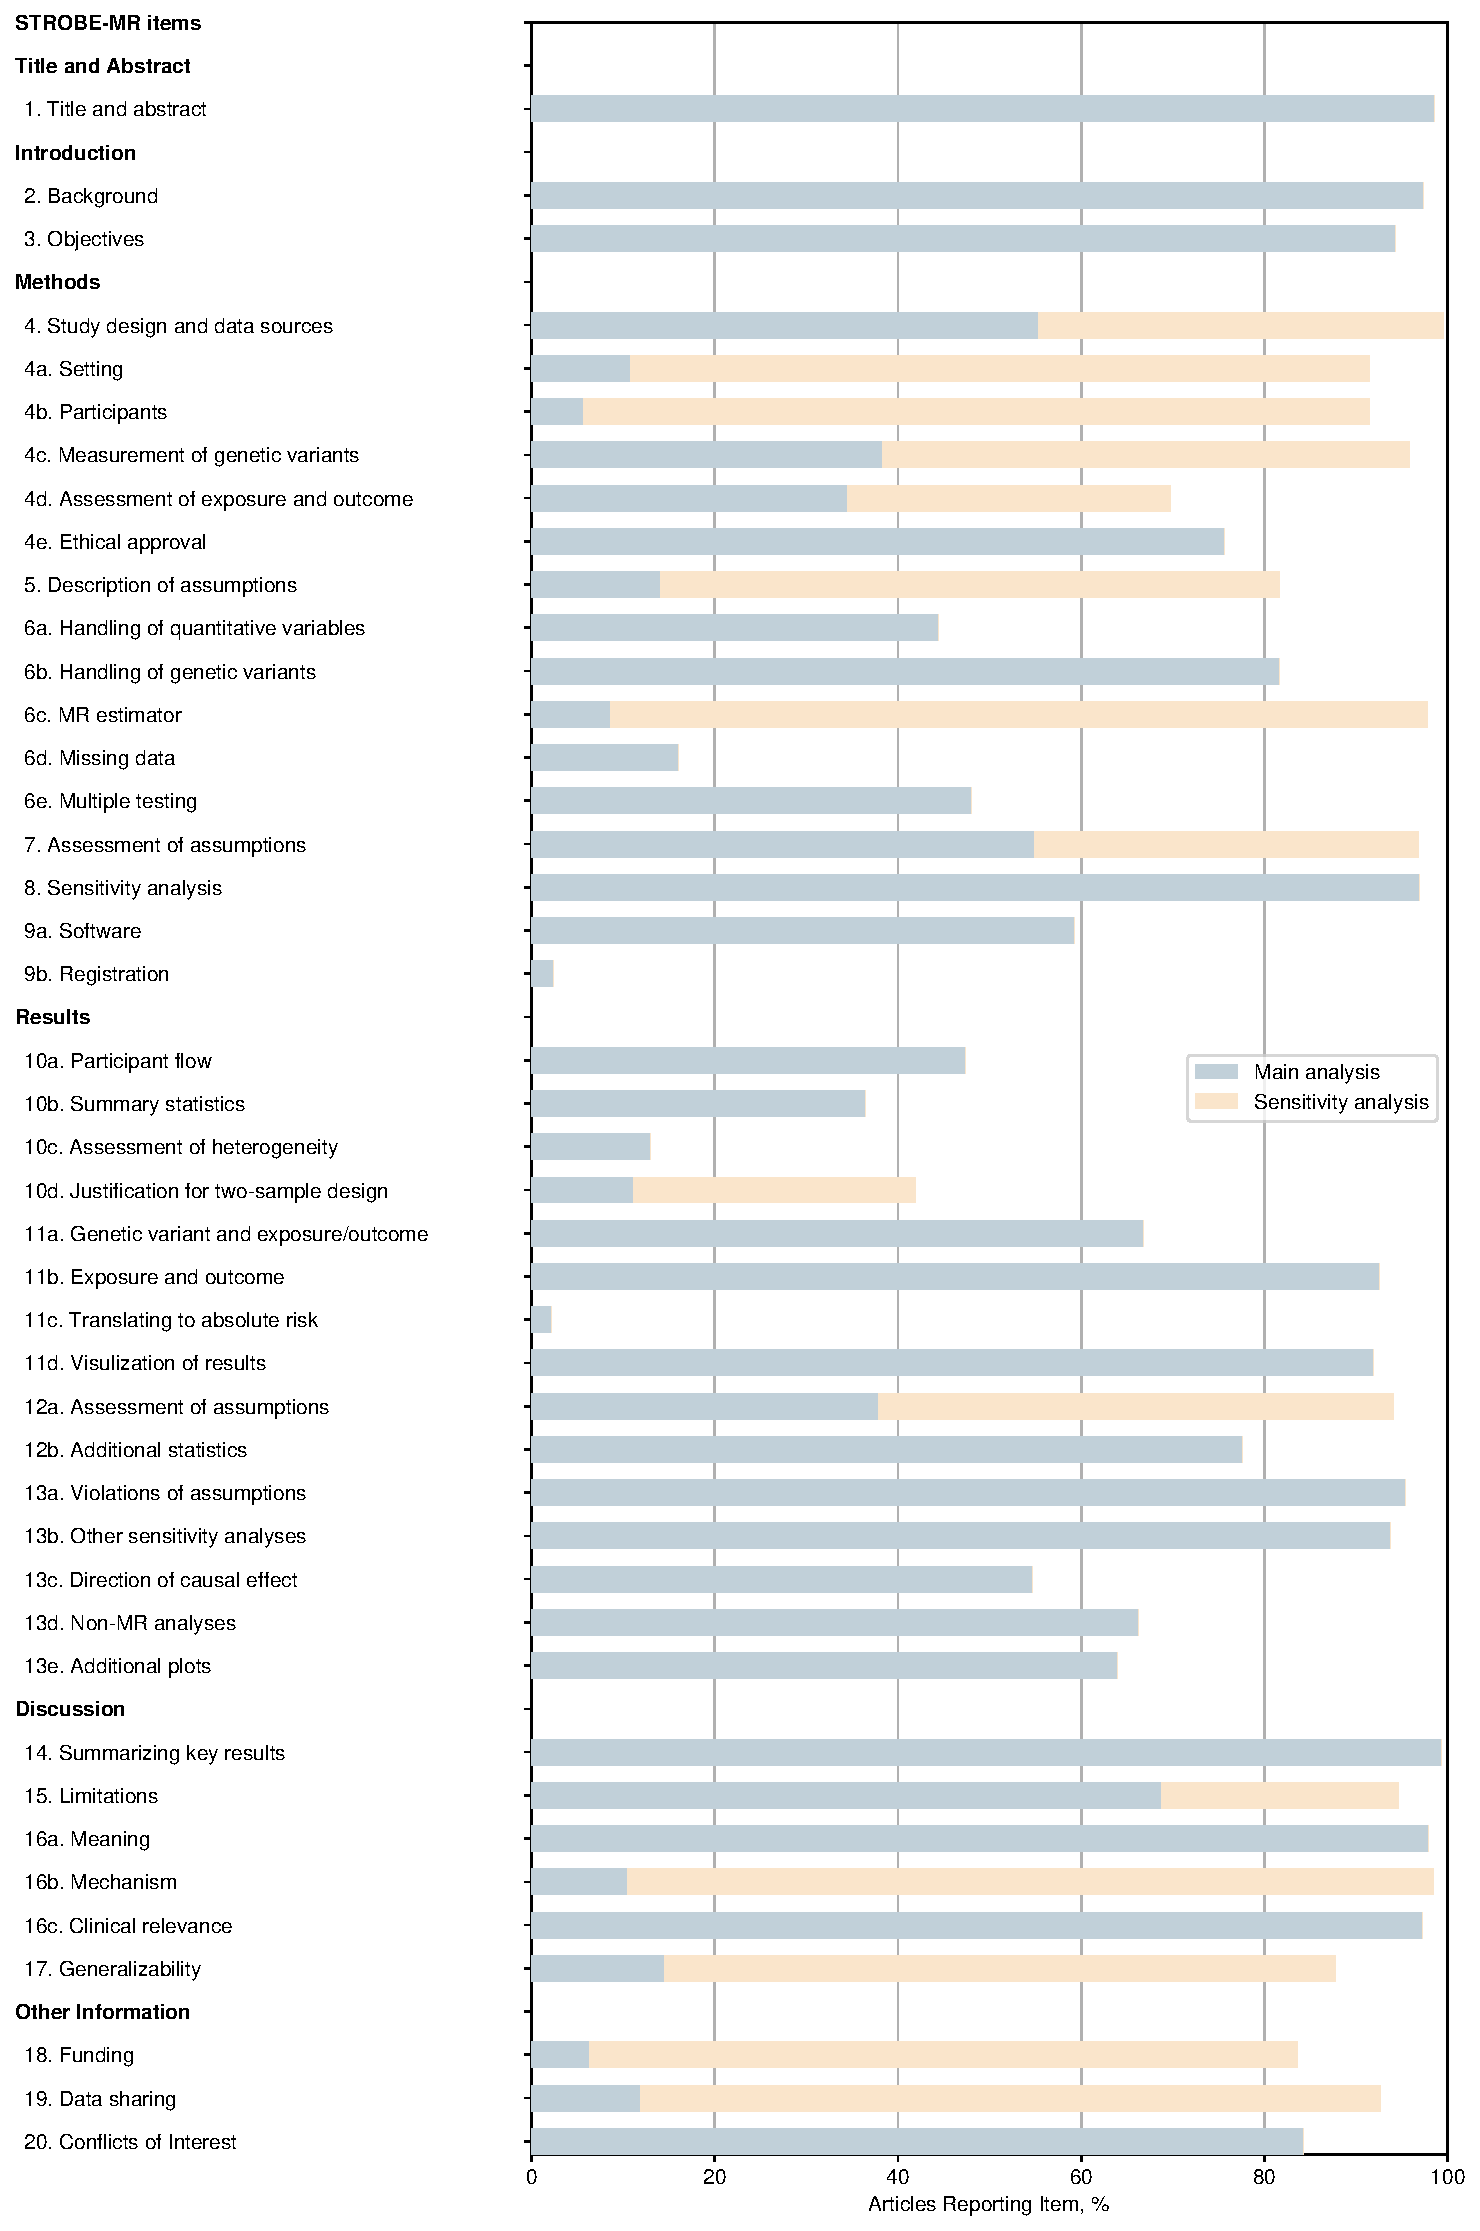
\includegraphics[width=0.8\linewidth]{assets/figures/subitem_any/meet_percentage_by_subitem.pdf}
    \caption{Sensitivity analysis: STROBE-MR reporting by item}
    \label{append:fig:meet:year}
\end{figure}

\begin{figure}[H]
    \centering
    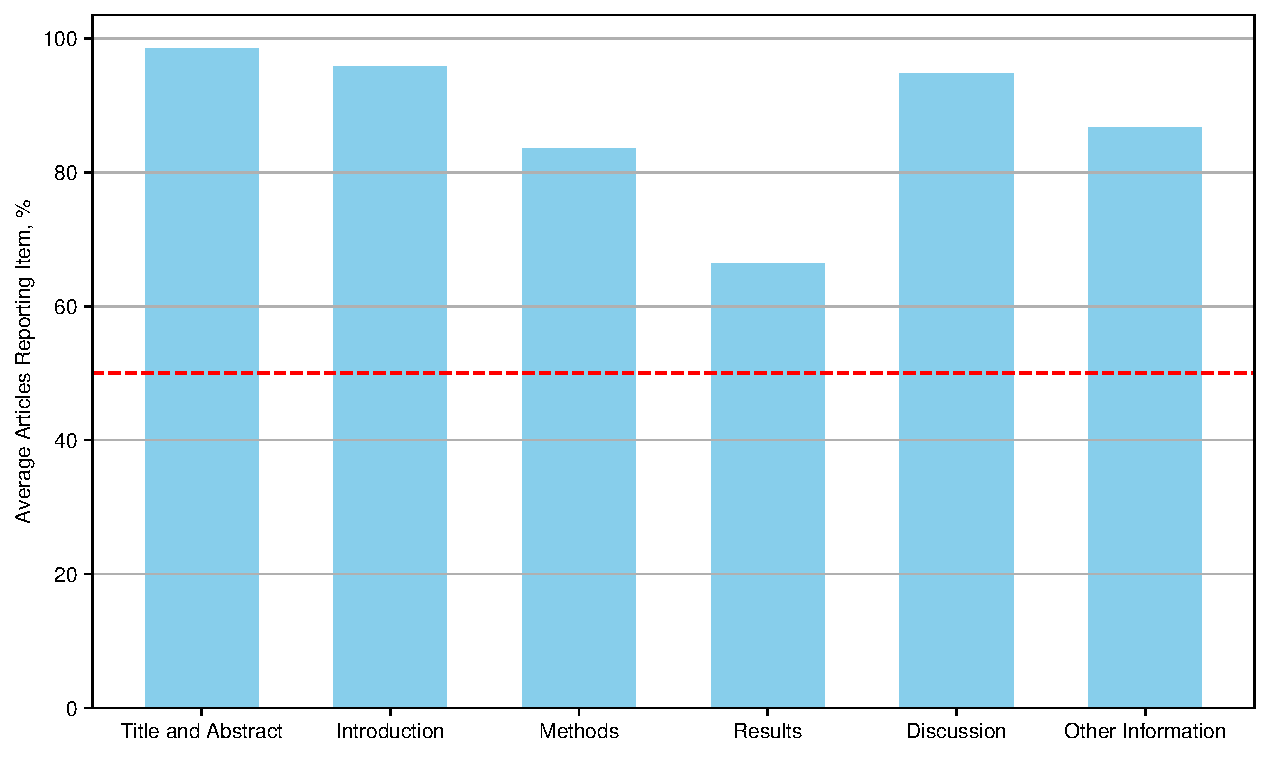
\includegraphics[width=0.8\linewidth]{assets/figures/subitem_any/meet_percentage_by_section.pdf}
    \caption{Sensitivity analysis: STROBE-MR reporting by section}
    \label{append:fig:meet:year}
\end{figure}


\begin{figure}[H]
    \centering
    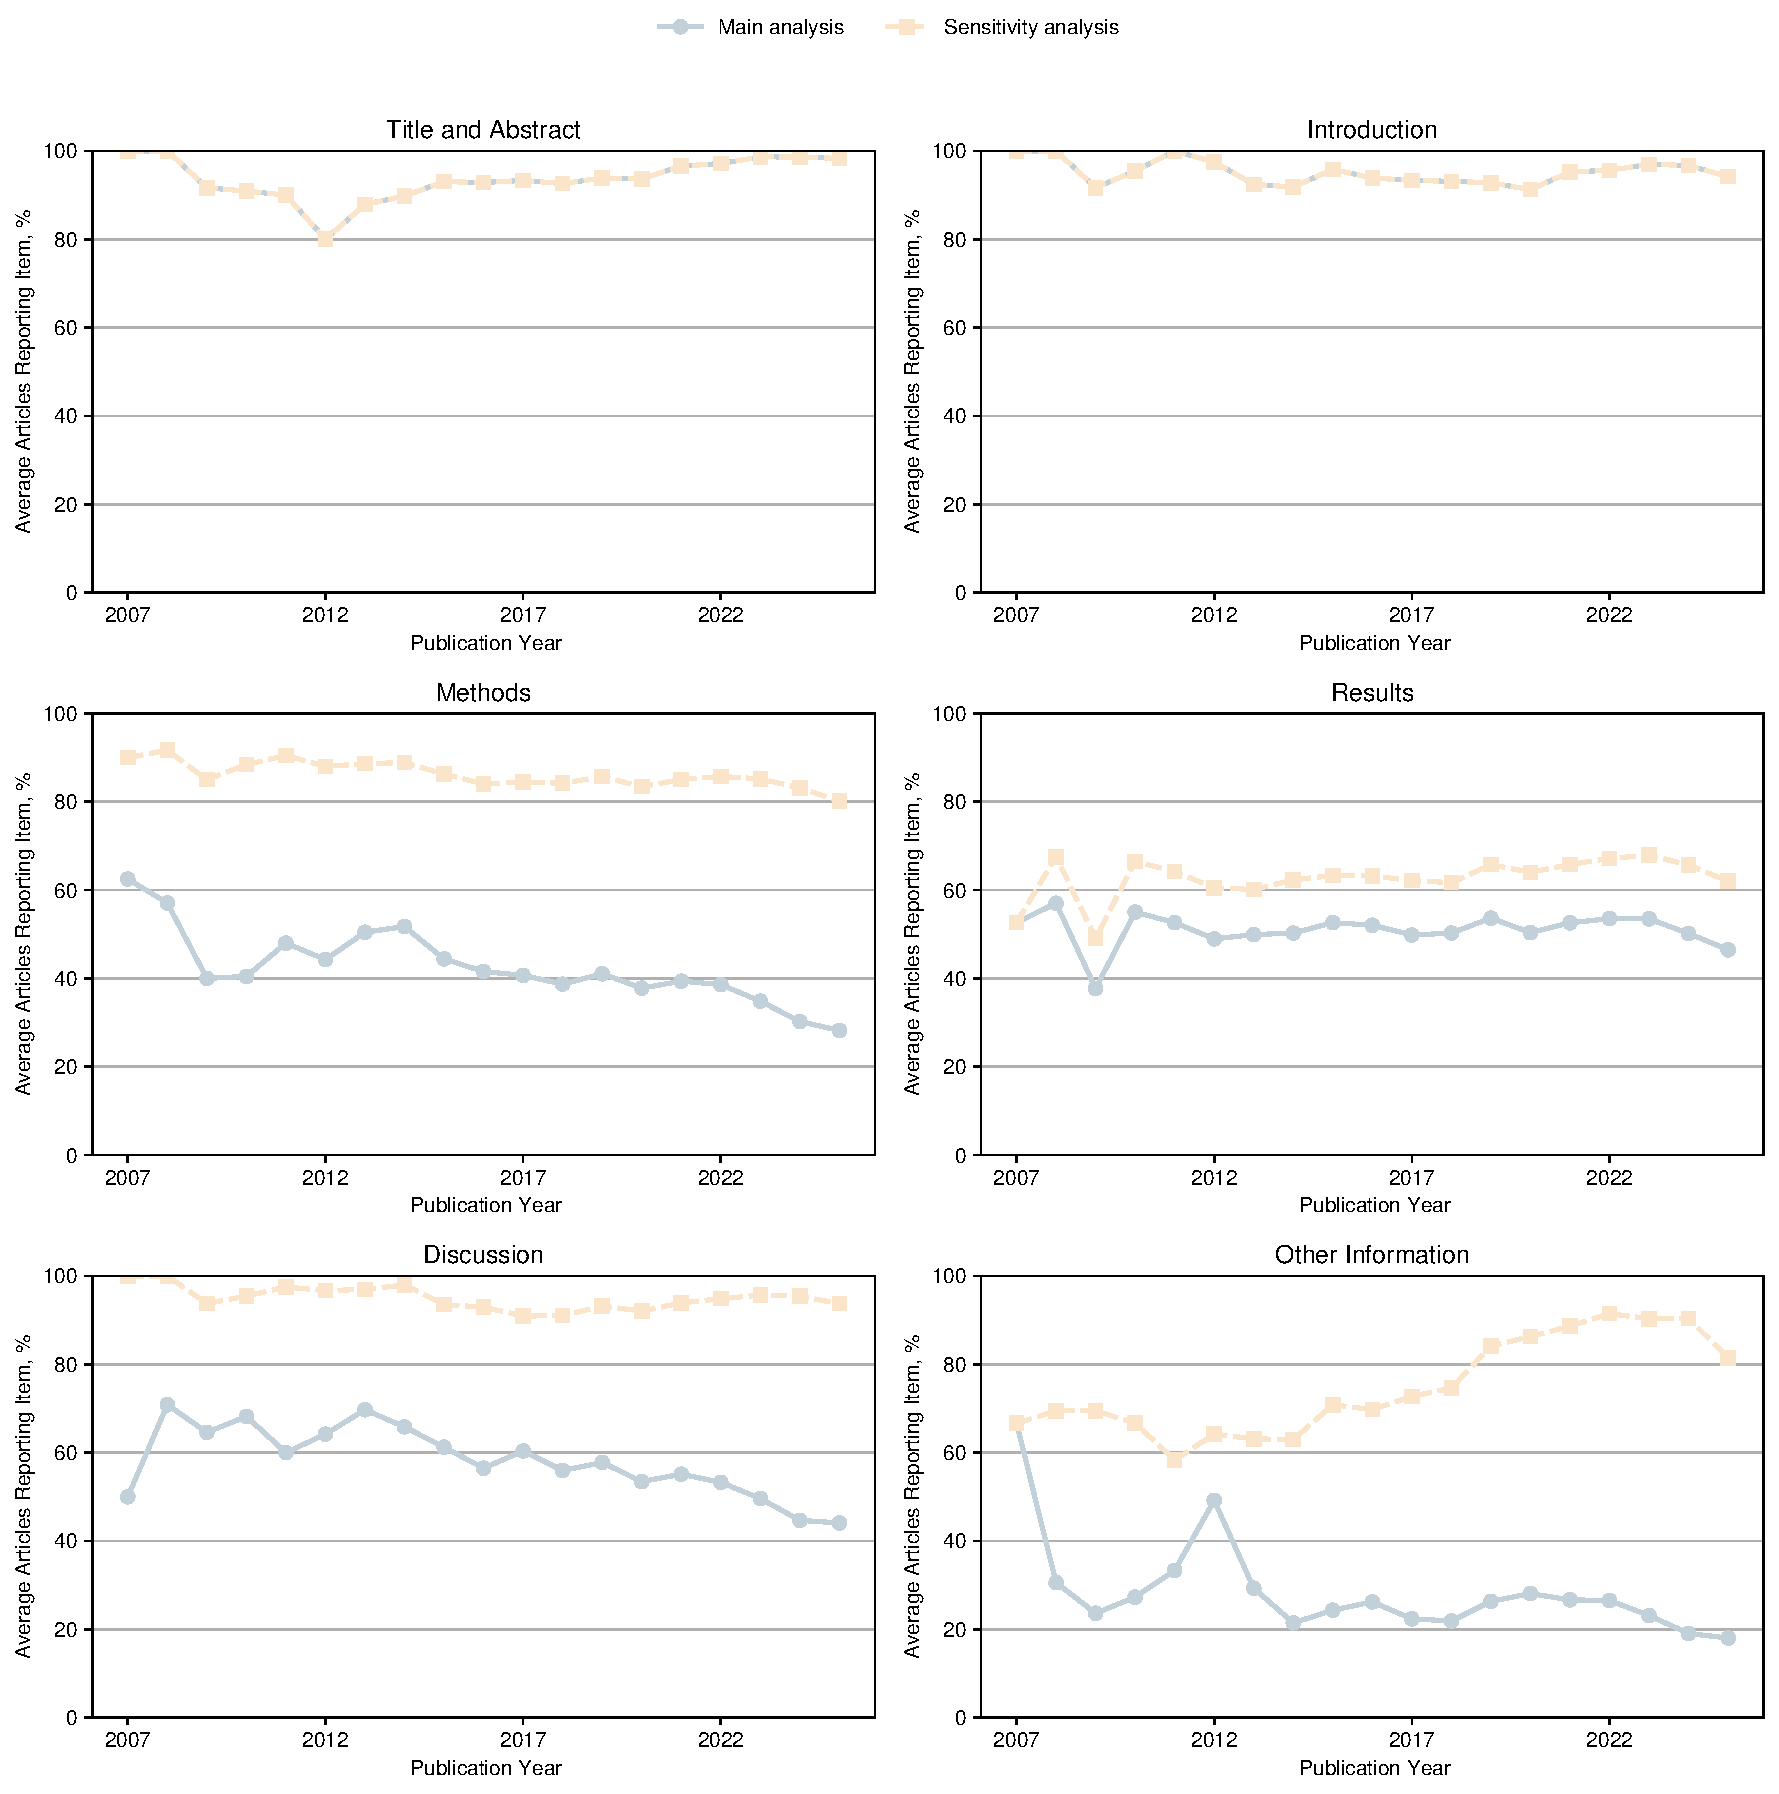
\includegraphics[width=0.8\linewidth]{assets/figures/subitem_any/meet_percentage_by_year_and_section.pdf}
    \caption{Sensitivity analysis: STROBE-MR reporting by year and section}
    \label{append:fig:meet:year}
\end{figure}

% Example cross-reference back to main manuscript
% This figure provides additional detail to Figure~\ref{fig:main-result} in the main manuscript.

\pagebreak

% ==== Optional: LLM declaration ====
% Uncomment if your target journal requires disclosure of LLM usage (increasingly common).
% \section{Declaration on the use of large language models} \label{sec:supp-use-of-llms}
% % Declaration on the use of large language models
% Many journals now require explicit disclosure of LLM usage.
% Adapt this section to accurately reflect your project's use.
% Reference policy: https://www.iscb.org/iscb-policy-statements/iscb-policy-for-acceptable-use-of-large-language-models

% [OPTIONAL] If LLMs were used in the research itself, describe that here:
In our work, as reported in the main text, LLMs were used as part of the research to assess reporting quality of MR studies.

% [OPTIONAL] If LLMs were used as coding/writing assistants, describe that here:
LLMs have been used as coding agents to assist:

\begin{itemize}
  \item for research analysis, the implementation of code (Python web crawler and annotation tools) and documentation;
  \item for the final proof-reading of the manuscript.
\end{itemize}

% coding agents
% List the coding agent tools used (e.g. GitHub Copilot, OpenCode, Cursor):
Coding agents used in our work include GitHub Copilot.
% models
% List the specific LLM models used:
The LLMs used include GPT-5 and Claude Opus 4.
% model access
% Describe how the models were accessed (API, web interface, IDE plugin, etc.):
The LLMs are accessed via API and IDE plugins.

% Describe provenance of figures and tables:
Figures and tables used in the manuscript are generated from analysis code
which AI was used in their implementation, but are not directly generated by AI.

% other tools
% List non-AI writing/proofreading tools used:
Other non-AI / non-LLM tools in proof-reading the manuscript include
textidote (\url{https://github.com/sylvainhalle/textidote}) and
typos (\url{https://github.com/crate-ci/typos}).

The final manuscript is fully drafted by the authors and has been reviewed and edited by all co-authors.
Prior to submission we have reviewed ISCB Policy for Acceptable Use of Large Language Models
(\url{https://www.iscb.org/iscb-policy-statements/iscb-policy-for-acceptable-use-of-large-language-models})
and follow its guidelines on the acceptable uses.

% \pagebreak

% Bibliography
\bibliography{bib}

\end{document}
